\documentclass[12pt]{article}
\usepackage{myart}
% \addbibresource{/Users/lwg342/Documents/LaTeX/lib.bib}
\addbibresource{lib1.bib}
\usepackage{booktabs}\usepackage{authblk}
\usepackage{longtable}
\usepackage{tabularx}
%--------Hello World--------%
%=====================================%
\begin{document}
    \title{Augment Large Covariance Matrix Estimation With Auxiliary Network Information}
    \author[]{Shuyi Ge\thanks{Author email:sg751@cam.ac.uk}}
    \author[]{Shaoran Li\thanks{Author email:sl736@cam.ac.uk}}
    \author[]{Oliver Linton\thanks{Author email:obl20@cam.ac.uk}}
    \author[]{Weiguang Liu\thanks{Author email:wl342@cam.ac.uk}}
    \affil[]{Faculty of Economics, University of Cambridge}
    \maketitle
    % \tableofcontents
    
    \begin{abstract}
        This paper aims to incorporate auxiliary information about the location of significant correlations into the estimation of high-dimensional covariance matrices. With the development of machine learning techniques such as textual analysis, granular linkage information among firms that used to be notoriously hard to get are now becoming available to researchers. Our proposed method provides an avenue for combining those auxiliary network information with traditional economic datasets to improve the estimation of a large covariance matrix. Simulation results show that the proposed adaptive correlation thresholding method generally performs better in the estimation of covariance matrices than previous methods, especially when the true covariance matrix is sparse and the auxiliary network contains genuine information. As a preliminary application, we apply the method to the estimation of the covariance matrix of asset returns. There are several extensions and improvements that we are considering.     
    \end{abstract}
    
    \section{Model and Introduction}Our goal is to estimate \(\Sigma =\variance(y)\) where \(y\) is a \(p \times 1\) random vector, say asset returns. We collect the \(T\) observations into a matrix \(Y:p\times T\). Sample covariance estimate \(\hat{\Sigma} = \frac{1}{T} (Y - \bar{Y}\mathbf{1})(Y - \bar{Y}\mathbf{1})'\) is problematic when \(p\) is not small relative to \(T\). Popular estimation strategies include factor model, shrinkage, thresholding, banding, tapering, etc.

If in addition to the observation of \(Y\), we observe a network \(G\) among the firms, where \(G_{ij}\) either takes value \(0,1\) or a score in \([0,1]\), with higher \(G_{ij}\) implying that it's more ``likely'' that the returns of firm \(i,j\) are correlated. We show that this auxiliary network can be used to improve the estimation the covariance matrix \(\Sigma\). Examples of such network include \cite{hoberg2016TextBasedNetwork}, who identifies a product similarity network from financial reports that has been shown to be more accurate than industry block diagonal matrix. As linked firms are potentially subject to similar demand shock, we have reason to believe that \(G\) contains valuable information about the comovement among the returns.
\cite{israelsen2016does} and \cite{kaustia2020CommonAnalysts} both find that companies covered by the same analysts show similarities in many unobserved dimensions, and this analyst-based network could explain excess co-movement on top of common factors. With the development of machine learning techniques such as textual analysis, we are better at acquiring information from big data. Granular linkage information among firms that used to be notoriously hard to get due to its proprietary properties,  now are becoming available to researchers. The question is, how to use those auxiliary network information to  better estimate the co-movement between assets?

% For example, such \(G\) information could come from textual analysis, that has become more and more popular in finance, for example (\cite{fan2021HowMuch}). 

This paper aims to provide ways to extract the information contained in the auxiliary \(G\) matrix to help estimate the covariance \(\Sigma\). We consider an \textit{Adaptive Correlation Thresholding} method, where we apply thresholding to the correlation matrix, with the threshold level depending on network information. More specifically, suppose we observe \(Y_{t}\) for \(t = 1 ,\dots, T\), the procedure is 
% \begin{enumerate}
    % \item 
    % \item Guided Linear Shrinkage: we adopt the linear shrinkage method, where the shrainkge targets is chosen based on the network information. This is different from previous practice of shrinking to the identity or equicorrelation matrix. 
% \end{enumerate}

\begin{enumerate}
    \item Estimate the sample covariance estimate \(\hat{\Sigma}\), and the sample correlation matrix \(\hat{R}\). 
    \item Apply the generalized thresholding function \(h(r_{ij},\tau_{ij})\) to the off-diagonal elements of \(\hat{R} = (\hat{r}_{ij})\), as in  \cite{rothman2009GeneralizedThresholding}. The novelty is now we allow the threshold \(\tau_{ij}\) to vary across elements and to depend on the network information.  Specifications we have considered for the threshold \(\tau\) are 
    \begin{itemize}
        \item Simple linear model 
            \begin{equation*}
                \tau(G_{ij}) = a + bG_{ij}
            \end{equation*}
        \item 
        The probit model
            \begin{equation*}
            \tau_{ij} = \tau\pqty{G_{ij}} = \Phi\pqty{a + b \abs{G_{ij}}}
            \end{equation*}
    \end{itemize}
    \item Estimate the unknown parameters in the \(\tau\) function by cross validation, as in \cite{bickel2008CovarianceRegularization}, \cite{cai2011AdaptiveThresholding}, where we randomly split the sample \(V\) times, for each \(v\), compute the new estimator \(\hat{\Sigma}^{1,v}_{G}\) with the first subsample, and sample covariance \(\hat{\Sigma}^{2,v}\) and the criterion is 
    \begin{equation*}
        L(a, b) = \frac{1}{V} \sum_{v}^{V} \norm{\hat{\Sigma}^{1,v}_{G} - \hat{\Sigma}^{2,v}}^{2}_{F}
    \end{equation*}
    we find \(a,b\) that minimise this criterion. 
    
    \item Then with the estimates of \(a,b\), we can estimate \(\Sigma\) on the test sample. 
\end{enumerate}

%For the second method we consider, we construct a linear shrinkage target based on the hard-thresholded version of \(\hat{\Sigma}\), call it \(\hat{\Sigma}_{H} = [\hat{\Sigma}_{ij} \mathbf{1}\Bqty{G_{ij} > 0}]\). And apply linear shrinkage with the target. 

There are several advantages of using network guided method:
\begin{enumerate}
    \item The main advantage is that we are combining economically meaningful network with market-based performance data. Comparing to purely data-driven thresholding or shrinkage methods, the method utilizes valuable information embedded in external network data, which provides more robustness and efficiency. aif our auxiliary network contains the ``real'' links from the network. The relationship identified will be more stable over time than the relationship identified from return data alone. 
    \item This method is very flexible and extensible. Although in our current analysis we only use one of the existing networks as our proxy for $G$, you are free to include many candidate networks in the \(\tau\). You may want want to include characteristics-based distances, as it has been documented that companies with similar characteristics exhibit additional co-movement on top of common risk factors (see \cite{fernandez2011spatial} for example). It also provides a way to discern which set of information is relevant based an estimate of the coefficients \(a,b\) in the thresholding level. 
    \item The networks may provide industry-level comovement that is potentially related to the ``weak factors'' components, which we intend to investigate. 
\end{enumerate}

% There are some challanges and questions as well:
% \begin{enumerate}
    % \item Since we don't observe the true \(\Sigma\), we wonder if there are some good criteria for evaluating the performance of our \(\hat{\Sigma}\). So far I am following \cite{ledoit2004HoneyShrunk} and \cite{ledoit2017NonlinearShrinkage}. But unlike the linear and nonlinear shrinkage method, our estimator is not designed for optimal performance under the Frobenius norm. 
    % \item We don't have a quality measure of the network matrix or a model for how the \(G_{ij}\) are generated. 
    % \item In simulation studies, the optimization takes some time, but the result is not yet very robust(some times it outperforms all competitors, but sometimes the optimization will be very   off-target).
% \end{enumerate}

    \section{Literature Review}    With the technology such as machine learning based textual analysis, we have acquired a lot of auxiliary information about the linkage between companies, industries and so on. Can we use that information to better estimate the co-movement between assets?

    Let \(Y = \pqty{Y_{1},\dots,Y_{p}}'\) be a random vector of excess returns, we want to estimate the covaraince \(\Sigma = \variance\pqty{Y}\). 

    \cite{bickel2008CovarianceRegularization} considers banding or tapering the sample covariance matrix. \cite{bickel2008CovarianceRegularization} considers covariance regularization by hard thresholding. 
    \begin{review}[\cite{bickel2008CovarianceRegularization}] 
        Define \(T_{s}(M) = \bqty{m_{ij} \mathbf{1}_{\abs{m_{ij} \geq s}}}\). Define the uniformity class for \(0 \leq q < 1\) 
        \begin{equation}
            \mathcal{U}_{\tau}(q,c_{0}(q),M) = \Bqty{\Sigma: \sigma_{ii}\leq M, \sum_{j}\abs{\sigma_{ij}}^{q}\leq c_{0}(p), \forall i}
        \end{equation}
        They show that for sufficiently large \(M'\), \(t_{n} = M'\sqrt{\frac{\log p}{n}} \) and \(\log p /n \to 0\), 
        \begin{equation}
            \hat{\Sigma} = \frac{1}{n} \sum_{k} \pqty{Y_{k} - \bar{Y}}\pqty{Y_{k} - \bar{Y}}'
        \end{equation}
        \begin{equation}
            \norm{T_{t_{n}}(\hat{\Sigma}) - \Sigma} = O_{p}\pqty{c_{0}(p) \pqty{\frac{\log p}{n}}^{(1-q)/2}}
        \end{equation}
    \end{review}


    \begin{review}[\cite{cai2011AdaptiveThresholding}]
        Adaptive thresholding where instead of doing \(T_{t_{n}}\), threshold as:
        \begin{equation}
            \hat{\sigma}_{ij}^{*} = s_{t_{ij}}\pqty{\hat{\sigma}_{ij}}
        \end{equation}
        where \begin{enumerate*}
            \item \(\abs{s_{\lambda}(z)} \leq c \abs{y}\) for all \(\abs{z - y}\leq \lambda\)
            \item \(s_{\lambda}(z) = 0\) for \(\abs{z}\leq \lambda\)
            \item \(\abs{s_{\lambda}(z) - z} \leq \lambda\).
        \end{enumerate*}

        The convergence rate is the same, although here the uniformity class is larger. 
    \end{review}
    \begin{review}[\cite{fan2016IncorporatingGlobal}]
        They use hard thresholding based on the sector/industry classifier. \(s_{ij}(\sigma_{ij})= \sigma_{ij}\) if \(ij\) are in the same industry. 

        And they are in a high-frequency setting. 
    \end{review}

    \cite{ledoit2004HoneyShrunk} develops an estimation strategy based on shrinkage. 
    \section{Simulations}Codes can be found here \href{https://github.com/lwg342/Covariance-Estimation-with-Auxiliary-Information}{Repo Link}
    \subsection{Simulation 1}
        We generate \(T = 100\) independent samples from \(p = 400\) dimensional normal distribution \(N(0, \Sigma_{1})\), where \(\Sigma_{1}\) is constructed by concatenating four AR(1) serial correlation matrix with ones on the diagonal and parameter \(\rho = 0.9\). The network \(G = [G_{ij}]\) where \(G_{ij} = 1\) if \(\sigma_{ij} > 0.6\). 
        
        Given the \(T = 100\) sample and the \(G\) matrix, we compute the correlation matrix \(R\) and apply the hard threshold function \(h(r_{ij}, \tau_{ij})\) to the off-diagonal elements of \(R\), that is 
        \begin{equation*}
            h(r_{ij}, \tau_{ij}) = r_{ij} \mathbf{1}\pqty{\abs{r_{ij}} > \tau_{ij} \& i \neq j}
        \end{equation*}
        the \(\tau_{ij}\) depends on \(G_{ij}\) and is specified here as probit function so that it's between \(0, 1\)
        \begin{equation*}
            \tau_{ij} = \Phi(a + b G_{ij})
        \end{equation*}
        
        The following \autoref{table:1} describes the Frobenius-norm error using different estimators, the new estimator which is optimized to minimise the Frobenius error, has good performance. 
         In \autoref{fig:1} we show the heatmaps of the true \(\Sigma\) and the estimates. Perhaps using a softer thresholding function will give better result. 2. We are trying more meaningful specification of \(\Sigma\) and we suspect that the new estimator will be good at preserving  important structural features of the covariance.
        
        \begin{table}[htbp]
            \centering
            \begin{tabular}{ll}
            New estimator               & 35.5759973173453  \\
            Linear shrinkage    & 36.44438551876532 \\
            Nonlinear shrinkage & 35.09953816084891 \\
            Sample              & 40.62939042523703 \\
            Sample - New        & 49.10202294326661
            \end{tabular}
            \caption{Difference with true \(\Sigma\) in terms of Frobenius Norm}
            \label{table:1}
        \end{table}
   
        \begin{figure}[tbp]
            \centering
            \makebox[\textwidth][c]{\includegraphics[width=1.8\textwidth]{Covariance-Estimation-with-Auxiliary-Information/asset/fig/Heatmap--2020112418.eps}}
            \caption{Comparison between the heatmaps of the matrices}
            \label{fig:1}
        \end{figure}        

        
        We have tried different specifications of the true \(\Sigma\) and repeated this calculation. For some specifications, the results are unstable: either it's difficult to find the minimum, or the result performs no better than the sample covariance estimate. I have also tried linear function \(\tau_{ij} = a + bG_{ij}\) and direct hard thresholding \(\tau_{ij} = G_{ij}\).  We are still improving the code for solving this model.
    \subsection{Simulation 2}
        Here we do a simulation on the case where \(G\) contains no real information. 
        
    \newpage
    \subsection{Empirical Study}
        We consider the estimation of covariance matrix among assets, where we supppose excess returns \(Y_{it}\) has a factor model + sparse structure:
        \begin{equation*}
            Y_{it} = B_{i} ' F_{t} + u_{it}
        \end{equation*}
        where \(\Sigma_{u}\) is assumed to be sparse. In addition to observaions of \(Y_{it}\) we have the similarity score network \(G\) from \cite{hoberg2016TextBasedNetwork}. Out of all pairs of assets, around \(2.5\%\) has score. We have matched the return data with the network and done the following
        
        \begin{enumerate}
            \item Compute the sample covariance matrix \(\hat{\Sigma}_{Y}\);
            \item Find the 3 largest eigenvalue \(\lambda_{1},\lambda_{2}, \lambda_{3}\) of \(\hat{\Sigma}_{Y}\) and the corresponding eigenvectors \(v_{1}, v_{2}, v_{3}\), and get \(\hat{\Sigma}_{u} = \hat{\Sigma}_{Y} - \sum_{k}^{3} \lambda_{k} v_{k} v_{k}' \)
            \item We compute the correlation matrix \(R_{u}\), and plot the density of the correlation coefficients \(r_{ij}\). 
            \item We compute the density of the correlation coefficient of \(r_{ij}\) for those \((i,j)\) pair that \(G_{ij} = 1\). 
        \end{enumerate}
        The result is the following two graphs. Both graphs don't include the diagonal \(1\)'s. 
        \begin{figure}[htbp]
            \centering
            \includegraphics{Covariance-Estimation-with-Auxiliary-Information/asset/fig/density-corr-plots-hoberg.eps}
            \caption{Density Plot of \(r_{ij}\) for \((i,j)\) that has link in Hoberg's Network}
            \label{<label>}
        \end{figure}

        \begin{figure}[htbp]
            \centering
            \includegraphics{Covariance-Estimation-with-Auxiliary-Information/asset/fig/density-corr-plots.eps}           
            \caption{Density Plots of \(r_{ij}\)}
        \end{figure}       

        We are still coding for the empirical estimation of the covariance, so no final result, but it seems that even after removing the factor component, there is some signal in the network information that we can use to estimate the covariance. 
    \section{Empirical Study}In this section, we apply the adaptive correlation thresholding method to a portfolio construction problem. First we describe the procedure and then present some of the results we have. 

Assume we observe the excess return \(Y_{it}\), \(i = 1,\dots,N\) and \(t= 1,\dots, T\) follows
\begin{equation*}
    Y_{it} = B_{i}' F_{t} + u_{it} ; \quad \Sigma_{u} = E(u_{t}u_{t}')
\end{equation*}
where \(F_{t}\) are factor excess returns. Here we have considered Fama-French 3 and the Carhart's momentum factor. The goal is to estimate \(\Sigma_{Y} = E\pqty{YY'}\) and use that estimate to construct portfolio following \cite{ledoit2017NonlinearShrinkage}. The auxialiary network we have include the \cite{hoberg2016TextBasedNetwork}'s network(henceforth Hoberg's Network) and IBES analysts cocoverage network. Here we present the results for SP500 returns using Hoberg's Network. 

The procedure we take is as follows. 
\begin{enumerate}
    \item We run time series linear regressions of \(Y_{it}\) on \(F_{k,t}\), obtain the beta estimates \(\hat{B}_{i}\) and the residual \(\hat{u}_{it}\). 
    \item Compute the covaraince matrix \(S_{\hat{u}} = \frac{1}{T}\hat{u}\hat{u}'\) and \(S_{F} = \frac{1}{T} \sum_{t} (F_{t} - \bar{F})(F_{t} - \bar{F})'\) and appply \textit{adaptive correlation thresholding} on \(S_{\hat{u}}\), denote the estimate as \(\hat{S}_{\hat{u}}\). 
where the second step adaptive correlation thresholding is achieved in the following way. Let \(R_{u}\) be the correlation matrix calculated from \(S_{u}\). We use soft thresholding \(h(r_{ij}, \tau_{ij}) = \sign\pqty{r_{ij}} \pqty{r_{ij} - \tau_{ij}}_{+}\) on the off-diagonal elemetns \(r_{ij}\) of \(R_{u}\), where 
\begin{equation*}
    \tau_{ij} = \delta_{ij} \sqrt{\frac{\log N}{T}}
\end{equation*}
and 
\begin{equation*}
    \delta_{ij} = a + b G_{ij}
\end{equation*}

% \blue{(so that the network is a little denser, and I have also considered specification of \(\delta\) as a probit model, but it complicates the optimization part because the constraint is nonlinear.)}. 

Let the threshold estimate be \(\hat{R}_{\hat{u}}(a,b)\), given \(a,b\), our estimate will be
\begin{equation*}
    \hat{S}_{\hat{u}} = \hat{S}_{\hat{u}}(a,b) = \diag(S_{\hat{u}})^{\frac{1}{2}} \hat{R}_{\hat{u}}\diag(S_{\hat{u}})^{\frac{1}{2}}
\end{equation*}

In order to guarantee positive definiteness, I follow the suggestion in \cite{fan2015OverviewEstimation} and \cite{fan2013LargeCovariance}, by first finding the minimum \(\underline{\delta}\) such that the \(\hat{S}(\delta, 0)\) has its smallest eigenvalue larger than \(0\) if we choose \(\tau_{ij} = \underline{\delta} \sqrt{\frac{\log N}{T}}\). 

Then \(a,b\) are estimated using cross-validation following \cite{bickel2008CovarianceRegularization} by randomly spliting the sample \(V\) times, for each \(v = 1,\dots,V\), compute the estimate \(\hat{S}^{1,v}_{u}\) with the first subsample, and sample covariance estimate \(\hat{\Sigma}^{2,v}_{u}\) with the second subsample and let the criterion function be
\begin{equation*}
    L(a, b) = \frac{1}{V} \sum_{v}^{V} \norm{\hat{S}^{1,v}_{u} - \hat{\Sigma}^{2,v}_{u}}^{2}_{F}
\end{equation*}
we find \(\hat{a},\hat{b}\) that minimise this criterion subject to the constraints:
\begin{align}
    0 \leq a \sqrt{\frac{\log N}{T}} &\leq 1 \\
    b \sqrt{\frac{\log N}{T}} &\leq 0 \\
    \underline{\delta} &\leq a + b 
\end{align}
\item Construct an estimate of \(\Sigma_{Y}\) by \(\hat{\Sigma}_{Y} = \hat{B}S_{F}\hat{B}' +\hat{S}_{\hat{u}}\)
\end{enumerate}

We have estimated the covariance matrices of SP500 stocks from 1996 to the end of 2017; using stock return data and Fama-French 3 factor returns \(F_{kt}, k =1,2,3\). We incorporate Hoberg's network \(G_{t}\) that are updated yearly into our estimation procedure. 

The Hoberg's Network is a yearly updated \(N\times N\) network with elements in \([0,1]\) with higher score \(G_{ij}\) reflecting potentially higher correlation between the \(i\)-th and \(j\)-th firms.


In Figure 1, we present the distribution, we present the distribution (blue) of sample covariance estimates \(S_{\hat{u}, ij}\) of residuals after regressing the the stocks returns on the Fama-French 3 factor for the stocks that haIn Figure 1, we present the distribution (blue) of sample covariance estimates \(S_{\hat{u}, ij}\) of residuals after regressing the the stocks returns on the Fama-French 3 factor for the stocks tsiduals after regressing the the stocks returns on the Fama-French 3 factor for the stocks that have no missing data in the dataset; alongwith the distribution of  sample covariance \(S_{\hat{u},ij}\) for those \(ij\) with \(G_{ij} > 0\) in the Hoberg's network. It's clear that the distribution is shifted to the right, implying that Hoberg's network can pick up information that are not explained by the factors. 

\begin{figure}[htbp]
    \centering
    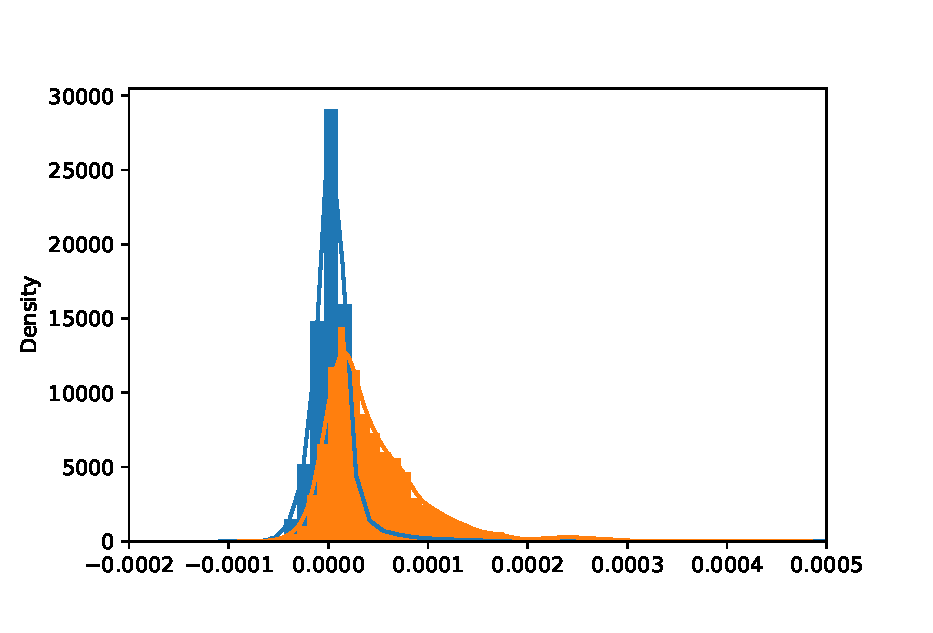
\includegraphics{fig1.eps}
    \caption{Distribution of \(S_{\hat{u},ij}, i,j = 1,\dots,N\) and \(S_{\hat{u},ij}\) for \(i,j\) such that \(G_{ij} >0\) }
    \label{<label>}
\end{figure}

Then we use a rolling-window estimation, with 252-day estimation period and then move the window forward by 21 days. In the estimation periods in window  \(m= 1, \dots,M\) we construct estimate \(\hat{\Sigma}_{Y,m} = \hat{B}S_{F}\hat{B}' + \hat{S}_{\hat{u}}\pqty{\hat{a}_{m}, \hat{b}_{m}}\). The estimated parameters \(\hat{a}_{m},\hat{b}_{m} \)  have mean \((1.177, -0.252)\), where the \(\hat{b}\) measures the effect of knowing the auxiliary network on the thresholding level. 

    \section{Conclusion and Further Works}This paper considers the problem of incorporating auxialiary data such as textual-analysis data into the estimation of large covariance matrices. It can be shown that by incorporating information about locations of important links we can relax the sparsity conditions of the thresholding estimators and in simulations we show the proposed Network Guided Estimator has superior performance in finite samples. We have also applied the Network Guided Estimator in the construction of minimum-variance portfolio in a preliminary empirical application. There are several improvements that we are undertaking.

Firstly, the construction of good estimator \(\hat{L}_{ij}\) for the important locations is an important question. It's apparent from the simulations that the quality of \(\hat{L}_{ij}\) will affect the estimation error. We have used a straightforward estimator in the empirical study, but it's not completely satisfactory and we need a more systematic way of constructing the \(\hat{L}\). Secondly, we are expanding the set of auxialiary networks beyond the RavenPack news data to include Hoberg's similarity score and IBES co-covarage data, as well as applying the technique on a larger dataset. 

% Firstly, we are applying the covaraince estimation technique on portfolio construction, following the problem considered in \cite{ledoit2004HoneyShrunk} and \cite{ledoit2017NonlinearShrinkage}, where the estimation of the sparse covaraince matrices are vital for constructing the minimum-variance portfolio. 

% Secondly, the method can be applied to study spatial-APT under large \(N\) case. \cite{kou2018AssetPricing} find that common risk factors are insufficient to capture all the significant inter-dependencies in asset returns, and local interactions are also important.  Spatial-APT and spatial CAPM type of models have not been popular in large N case since the measure of contiguity is challenging. Our method can uncover contemporaneously correlated entities by combining market-based information and auxiliary network information, thus providing a natural contiguity measure. Relying solely on either statistical methods or external network information is not as desirable as the links identified by the former are hard to interpret and the external network may miss some important links.



Although here we use network information to the estimation of large static covariance matrix, similar ideas can be extended to the estimation of large dynamic covariance matrix. For example, dynamic network information could be incorporated into the conditioning information set like in \cite{chen2019new}.


    % \section{Log}% \subsection{2020-08-21}
Can we build a full probability model for such problem. Suppose that \(y: {\Omega}\to \mathbb{R}^{p}\) be a random vector that has finite second moment. 
\begin{equation}
    \Sigma = \variance(y) = \bqty{\sigma_{ij}}_{i,j = 1,\dots,p}
\end{equation}

Suppose there is an observation matrix \(G_{t} = \bqty{g_{ij}}_{ij, t}\) for each time \(t\). 
\begin{equation}
    g_{ij,t} = \Phi\pqty{\theta_{1} \rho_{ij} + f(z_{i},z_{j})}
\end{equation}
where \(\rho_{ij}\) is the correlation coefficient. 
We can estimate \(\theta_{1}\) and \(f\) is a symmetric function, it could be \(\theta_{2} (z_{i} + z_{j})\), and \(z\) are asset characteristics such as size: larger firms have more media exposure. 

How to combine the two sets of information. Assume a DCC dynamic:
\begin{equation}
    \Sigma_{t} = D_{t}^{\frac{1}{2}} R_{t} D_{t}^{\frac{1}{2}}
\end{equation}
where \(D_{t}\) individually follows GARCH(1,1), \(R_{t}\). 

In DCC, \(R_{t}\) is written as \(r_{ij,t} = \frac{q_{ij,t}}{\sqrt{q_{ii,t} q_{jj,t}}}\) where \(q_{ij,t}\) follows GARCH, or exponential smoothing. 
\begin{equation}
    q_{ij,t} = \bar{\rho}_{ij,t} + \alpha \pqty{\epsilon_{i,t-1} \epsilon_{j,t-1} - \bar{\rho}_{ij}} + \beta \pqty{q_{ij,t} - \bar{\rho}_{ij}} 
\end{equation}

\subsection{2020-08-22}
I have tried to simulate covariance matrix, see simulation codes. Notice that in Bickel and Levina, they showed that banding is more efficient when the index has meaning.

Really it's about the model for \(g_{ij} = \mathbf{1}\pqty{\rho_{ij} > \tau}\). 
\begin{equation}
    P(g_{ij} = 1) = \Phi\pqty{\theta_{1}\rho_{ij} + \theta_{2} z_{1} + \theta_{3}z_{2}}
\end{equation}

Then we choose that \(\tilde{\rho}_{ij}\) that are significantly nonzero. 


\subsection{2020-09-01}
Based on the projection idea, suppose we have several estimator \(S_{1},\dots,S_k\) that besides the sample covariance matrix \(S_{0}\), we want to project \(\Sigma: n\times n\) from observations over \(t =1 ,\dots,T\) on \(I, S, S_{1},\dots S_{k}\). Suppose \(k = 1\), then we want to find the projection with the inner product defined on the space of random matrices :
\begin{equation}
    \ip{A}{B} = E \frac{1}{n} \tr[AB^{\top}]
\end{equation}

Then we have \(\Sigma = aI + \beta_{0}S_{0} + \beta_{1}S_{1}\), the oracle coefficients are 
\begin{equation}
    \bmqty{a \\ \beta_{0} \\\beta_{1}} = \bmqty{\norm{I}^{2} & \ip{S_{0}}{I} & \ip{S_{1}}{I} \\ \ip{I}{S_{0}} & \norm{S_{0}}^{2} & \ip{S_{1}}{S_{0}} \\ \ip{I}{S_{1}} & \ip{S_{0}}{S_{1}} & \norm{S_{1}}^{2} }^{-1}
    \bmqty{ \ip{\Sigma}{I} \\ \ip{\Sigma}{S_{0}}\\ \ip{\Sigma}{S_{1}}}
\end{equation}

Each quantity can be estimated by the sample counterpart, i.e. replacing \(\Sigma\)  with \(S_{0}\). We do a simulation.

But this is wrong, because we almost always fully load on the sample covariance matrix. I think it's because we can't simply replace the quantities with sample counterparts.

Suppose we have two estimators \(S_{1}, S_{2}\) for \(\Sigma\), we want to find \(\Sigma^{*} = \alpha I +\sum_{j}\beta_{j}S_{j}\) such that \(E \norm{\Sigma^{*} - \Sigma}^{2}\) is minimised. 

\begin{align}
    E \norm{\Sigma^{*} - \Sigma}^{2} = E\ip{ \alpha I +\sum_{j}\beta_{j}S_{j} - \Sigma}{\alpha I +\sum_{j}\beta_{j}S_{j} - \Sigma} 
\end{align}

Define 
\begin{align}
    \mu := \ip{\Sigma}{I} = E \ip{S_{1}}{I} =: \mu_{1}\\
    \mu_{2} := E \ip{S_{2}}{I} = E\bqty{\frac{1}{n} \tr S_{2,n}}
\end{align}

\red{Need to think about what can and cannot be directly estimated}
\subsection{2020-09-03}

We have on the LHS: 
\begin{equation}
    \bmqty{\ip{\Sigma}{I} \\\ip{\Sigma}{S_{1}} \\ \ip{\Sigma}{S_{2}}}
\end{equation} 
which involves unknown quantity \(\Sigma\).

\begin{align}
    \ip{\Sigma}{I}& = E \ip{S}{I} = E \frac{1}{n} \tr(S) \\
    &= \frac{1}{n} E \tr(\frac{1}{T} \sum x_{t}x_{t}')
\end{align}
which can be estimated with 
\begin{equation}
    \frac{1}{n} \frac{1}{T} \tr \pqty{\sum_{t} x_{t} x_{t}'}
\end{equation}

\subsection{2020-09-04}
The linear shrinkage is just projection with the inner product defined by \(\ip{A}{B}_{E} = E \ip{A}{B}\) for \(A, B\) random matrices taking value in the space of psd real matrices. 

\subsection{2020-10-10}:
Now lets consider if we can estimate the inner product between \(\Sigma\) and a another matrix \(A\), for which we have repeated observations such as the sample covariance \(S\). 

Let there be \(y_{t}: t = 1,\dots,T\), then we have 
\begin{equation*}
    S_{t} = y_{t} y_{t}' \qq{and} S = \frac{1}{T} \sum^{T} S_{t}f
\end{equation*}

The inner product is defined on random matrices: 
\begin{defn}
    Let \(A, B\) be random \(n\times n\) matrices, define 
    \begin{equation*}
        \ip{A}{B} = E \frac{1}{n} \tr(AB')
    \end{equation*}
\end{defn}

Then we can estimate \(\ip{\Sigma}{I} = E \frac{1}{n} \tr\pqty{\Sigma}\) by
\begin{equation*}
    \frac{1}{T} \sum_{t} \frac{1}{n}\tr\pqty{S_{t}}
\end{equation*}

For \(\ip{\Sigma}{S} = E \frac{1}{n} \tr\pqty{\Sigma S'}\), 
\begin{align*}
    \ip{\Sigma}{S} &= E \frac{1}{n} \sum_{i}\sum_{j} \sigma_{ij}s_{ij} \\
    &=  \frac{1}{n} \sum_{i}\sum_{j} \sigma_{ij}^{2}\\
    &= \ip{\Sigma}{\Sigma}
\end{align*}

\(\ip{\Sigma - S} = \norm{\Sigma}^{2} - \ip{S}{\Sigma} - \ip{\Sigma}{S} + \norm{S}^{2} = \norm{S}^{2} - \ip{\Sigma}{S}\). 

For the part
\begin{align}
    \norm{S}^{2} &= E \frac{1}{n} \sum_{i} \sum_{j} s_{ij}^{2} \\
    &= \frac{1}{n} E \sum_{i}\sum_{j} \pqty{\pqty{s_{ij} - \sigma_{ij}}^{2} + \sigma_{ij}^{2} } \\
    &= \frac{1}{n} \sum_{i}\sum_{j}E \pqty{\frac{1}{T} \pqty{\sum_{t} y_{it}y_{jt}'} - \sigma_{ij}}^{2} + R
\end{align}
the first term is just the variance of \(s_{ij}\) which is an estimate of \(\sigma_{ij} =  \covariance(y_{i}, y_{j})\). We can estimate it with:
\begin{equation*}
    \frac{1}{T} \pqty{\sum_{t} s_{t,ij} - s_{ij}}^{2}
\end{equation*}

Then consider a general \(A\):
\begin{align*}
    \ip{\Sigma}{A} &= \frac{1}{n} \sum_{i}\sum_{j} \sigma_{ij}a_{ij} \\
    &= \frac{1}{n} \sum_{i}\sum_{j} \sigma_{ij} E\pqty{a_{ij}}
\end{align*}

What's important is when \(a_{ij}\) and \(s_{ij}\) are not independent and when \(a_{ij}\) are not unbiased.
\subsection{2020-10-16}
Imagine the eigendecompositon, we are finding rank \(k\) approximation of \(\Sigma\). With the information in \(G\), suppose we have 
\begin{equation*}
    \norm{\Sigma - \Sigma \mathbf{1}_{G}} \qq{is small.}
\end{equation*}

Then \(G\) contains information that's useful.
\subsection{2020-11-09}
There are several questions:
\begin{enumerate}
    \item Does the network informs about the comovement?
    \item Now I think the best way is to combine the factor model, the shrinkage method and the network information. 
\end{enumerate}

\subsection{2020-11-12}

A network of cointegration relationship. 

\subsection{2020-11-18}
    Suppose we have a sparsity matrix to estimate, if we have some information about which location has zero elements: \(\sigma_{ij} = 0\), suppose this information is independent across \(ij\). Our estimate \(S^{*} = [S^{*}_{ij}]\) will try to minimise the Frobenius Norm: 
    \begin{equation*}
        \min E \sum_{i}\sum_{j} \pqty{\sigma_{ij} - s^{*}_{ij}}^{2}
    \end{equation*}
    
    Suppose we know the probability of \(\sigma_{ij} \neq 0\): \(p_{ij} = p(G_{ij}, X_{i}, X_{j})\) exactly, then suppose our sample estimation is \(s_{ij}\), for each element the expectation of MSE is:
    \begin{equation*}
        p_{ij} E (s_{ij} - \sigma_{ij})^{2} + (1-p_{ij}) E \pqty{s_{ij}^{2}} = E\pqty{s_{ij} - \sigma_{ij}}^{2}
    \end{equation*}
    if we use \(s_{ij}\) to estimate \(\sigma_{ij}\), the MSE of using \(0\) as estimate is:
    \begin{equation*}
        p_{ij} \sigma^{2}_{ij} 
    \end{equation*}
    so we would include \(s_{ij}\) if \(p_{ij}> \frac{E\pqty{s_{ij} - \sigma_{ij}}^{2}}{\sigma^{2}_{ij}}\)
    
    \subsection{2020-11-18}
    I have moved the original introduction section here. 
    \begin{question}
        Can we incorporate the information from \(G\) in the estimation of \(\Sigma\). I have thought of several ways:
    \end{question}

    \begin{enumerate}
        \item \textbf{Hard thresholding}: suppose we estimate the elements \(\sigma_{ij}\) in  \(\Sigma\) with \(s_{ij,G}(\hat{\sigma}_{ij})\), where \(\hat{\sigma}_{ij}\) are the sample covariance estimates, and \(s_{ij,G}\) is a hard-thresholding operator:
        \begin{equation}
            s_{ij,G}(\hat{\sigma}_{ij})
            \begin{cases}
                \hat{\sigma}_{ij} \qq{if} G_{ij} =1 \qq{or} i=j \\
                0 \qq{otherwise}
            \end{cases}
        \end{equation}

        Let the estimated matrix be \(\hat{S}_{G} = \pqty{s_{ij,G}(\hat{\sigma}_{ij})}_{i,j = 1,\dots, N}\). 
        \cite{bickel2008RegularizedEstimation} compares the difference between thresholding and banding and finds intuitively that if the assets are ordered in a meaningful way, then banding is more efficient than thresholding. Our method is like banding with ``order'' implied by \(G\). 

        \cite{fan2016IncorporatingGlobal} considers the hard thresholding where they only keep the \(\hat{\sigma}_{ij} \) for which \(i,j\) are in the same industry, so their \(G\) is just a block diagonal matrix. I think it will miss some important links. 

        \item \textbf{Shrinkage}: \cite{ledoit2004WellconditionedEstimator} considers finding a linear combination of sample covariance matrix \(\hat{\Sigma}\) and the shrinkage target \(I\) that minimizes the mean squared estimation error in Frobenius norm:
        \begin{equation}
            \min_{\rho_{1},\rho_{2}} E\pqty{\norm{\Sigma^{*} - \Sigma}^{2}} \qq{where} \Sigma^{*} = \rho_{1} \hat{\Sigma} + \rho_{2} I 
        \end{equation}

        I wonder if it makes sense to shrink towards hard-threshold estimator \(\hat{S}_{G}\), that is we find a minimizing linear combination:
        \begin{equation}
            \rho_{1}\hat{\Sigma} +\rho_{2}\hat{S}_{G} \qq{or} \rho_{1}\hat{\Sigma} +\rho_{2}\hat{S}_{G}  + \rho_{3} I
        \end{equation}

        \item A more direct approach:
        \begin{equation*}
            y_{it} = b_{i}'f_{t} + u_{it}
        \end{equation*}
        such that \(\Sigma_{u} = \Sigma_{G} + \Sigma_{u_{d}}\), that is after taking out the network component, the rest is a sparse matrix. 
    \end{enumerate}

    \begin{question}
        A related question is
        \begin{enumerate}
            \item How much information is contained in \(G\)? I thought about modeling a probit model, say
            \begin{equation}
                P(G_{ij} =1) = \Phi(\theta_{1} \sigma_{ij} +  f(z_{i},z_{j}))
            \end{equation}
            where \(z_{i}\) can be some firm characteristics such as \textit{size}: larger firms have more chances to be on the newspapers, and it's more likely to be linked to other firms. Maybe instead of hard threshold, we can do some weighting with weights calculated from \(\theta\).
        \end{enumerate}
    \end{question}
    
    \subsection{2020-11-19}
        Let's consider things we can do as a general plan for the python file. Suppose we have data \(X: T\times N\), from which we can calculate the sample covariance matrix \(S\) and the correlation matrix \(R\). 

        \subsubsection{Adaptive Correlation Thresholding}
        Suppose we use \textit{generalized thresholding operator} on \(R\): \(h(r,\tau)\) where several possibilities exist:
        \begin{enumerate}
            \item Hard thresholding: \(h(r,\tau) = r\) iff \(r \leq \tau\) or \(r\) is on the diagonal. 
            \item Soft thresholding: \(sign(r)(\abs{r} - \tau)_{+} \)
            \item SCAD, etc
        \end{enumerate}
        
        The \(\tau\) can be generated by 
        \begin{enumerate}
            \item Directly using \(G\), c.f. Hoberg's data.
            \item Use a probit model with \(G\). 
            \begin{equation}
                \tau\pqty{G_{ij}} = \Phi\pqty{a + b \abs{G_{ij}}}
            \end{equation}
            \item etc
        \end{enumerate}
        
\subsection{2020-11-24}
    If we have in addition to \(Y_{t}\) observations, some additional information \(G\) about the covariance \(\Sigma\). Can we improve the efficiency of estimating \(\Sigma\); can we relax the condition on how sparse the matrix is?

    For example, suppose we observe an estimated network  \(G: p \times p\) where \(g_{ij} = 1\) indicates that with probability \(p\), \(\sigma_{ij} > 0\) (or \(\sigma_{ij} > \tau\) for some level \(\tau\)). If \(g_{ij} =0\), then we have no information about \(\sigma_{ij}\). 

    With the additional information about \(G\), we can allow for a combination of
    \begin{enumerate}
        \item Dominant units that are correlated with many other assets, but the total number of dominant units is small;
        \item Block dependence among some units; 
        \item Sparse dependence of all the other assets on the previous two classes. 
    \end{enumerate}

    Let \(\mathcal{I}_{G}\subset \Bqty{1,\dots,p}\) be the index of stocks \(i\) such that \(\sum_{j} g_{ij} > 0\). Let \(p_{G} := \abs{\mathcal{I}_{G}}\) be the number of such stocks. 

    \begin{remark}
        We can extend it to consider all the connected nodes that are separated. Or even come up with a classifier. 
    \end{remark}

    Suppose \(p_{G}\) is small, then we can consistently estimate the matrix \(\Sigma_{G} = \variance\pqty{Y_{\mathcal{I}_{G}}}\) by 
    \begin{equation}
        \hat{\Sigma}_{G} := \frac{1}{T} \sum_{t} \pqty{Y_{t,\mathcal{I}_{G}} - \bar{Y}}\pqty{Y_{t,\mathcal{I}_{G}} - \bar{Y}}'
    \end{equation}
    \textbf{archive}:
    I have done some simulation with randomly generated sparse covariance matrix using three estimation methods, please see the html file for more details. 
    \begin{enumerate}
        \item Sample covariance matrix \(\hat{\Sigma}\);
        \item Ledoit-Wolf Shrinkage covariance matrix \(\Sigma^{*}\).
        \item Hard-thresholding matrix \(\hat{S}_{G}\).
    \end{enumerate}

    We randomly generate a sparse p.d. matrix \(\Sigma\) with dimension \(N\times N\), and for some fixed value \(\tau\), we observe \(G\) such that \begin{equation}
        G_{ij} = 1 \qq{if} \sigma_{ij} > \tau 
    \end{equation}
    In the simulation, we take \(N = 100\), and \(\tau\) is chosen such that 0.7\% of elements of \(G\) are \(1\). We draws \(T = 100\) iid sample from \(N(0,\Sigma)\), and estimate with the three methods.

    We find that \(\hat{S}_{G}\) does better in terms of matrix \(1\)-norm, and slightly worse in terms of Frobenius norm than \(\Sigma^{*}\), while both do much better than sample \(\hat{\Sigma}\). 


    \subsection{Empirical Study}
    In the empirical study, suppose a factor model for the asset returns
    \begin{equation*}
        Y_{it} = B_{i}'F_{t} + u_{it}
    \end{equation*}
    where \(\Sigma_{u}\) is assumed to be sparse. We consider the estimation of \(\Sigma_{u}\). 
    
\subsection{2020-01-03}
    The \(\lambda\) comes from a maximal inequality of Gaussian variables, from \cite{buhlmann2011StatisticsHighdimensional}:
    \begin{equation*}
        
    \end{equation*}
% The End
\printbibliography
\end{document}